
\subsection*{Opgave 1}
\stepcounter{section}
Vi skal bevise følgende sætning. 
\begin{setn}[Volumen af omdrejningslegeme]
	For en kontinuert funktion $f$ er volumen af omdrejningslegemet på intervallet $[a,b]$ givet ved
	\begin{align*}
		\pi \int_a^b(f(x))^2 dx.	
	\end{align*}	 
\end{setn}
	\begin{figure}[H]
	\centering
	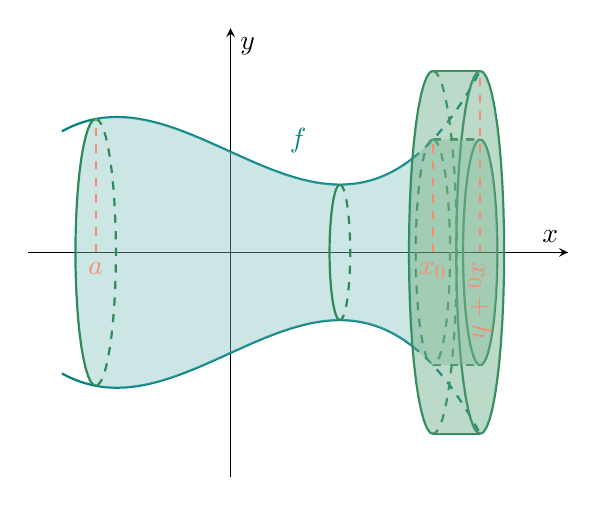
\begin{tikzpicture}
	\begin{axis}[
	axis lines = center, 
	xmin = -3, xmax = 5,
	ymin = -6, ymax = 6,
	ticks = none,
	xlabel = $x$, ylabel = $y$
	]
		\addplot[color = teal, thick, domain = -2.5:2.7, samples = 500] {0.1*x^(3) + 0.01*x^(2) - 0.82*x + 2.69};
		\addplot[color = teal, thick, domain = -2.5:2.7, samples = 500] {-(0.1*x^(3) + 0.01*x^(2) - 0.82*x + 2.69)};
		\addplot[color = teal, thick, domain = 2.7:3.7, samples = 200, dashed] {0.1*x^(3) + 0.01*x^(2) - 0.82*x + 2.69};
		\addplot[color = teal, thick, domain = 2.7:3.7, samples = 200, dashed] {-(0.1*x^(3) + 0.01*x^(2) - 0.82*x + 2.69)};
		\draw[] (axis cs: 3,0) -- (axis cs: 5,0);
		\node[color = teal] at (axis cs: 1,3) {$f$};
		%Filling
		\fill[color = teal!50, opacity = 0.4] 
		plot[domain = -2:3, variable = \x] (axis cs: \x, {0.1*(\x)^3 + 0.01*(\x)^2 - 0.82*\x + 2.69}) --
		plot[domain = 90:270, variable = \t] (axis cs: {0.254*cos(\t) + 3} , {151/50 * sin(\t)}) -- 
		plot[domain = 3:-2, variable = \x] (axis cs: \x, {-(0.1*(\x)^3 + 0.01*(\x)^2 - 0.82*\x + 2.69)}) --
		plot[domain = 270:90, variable = \t] (axis cs: {0.3*cos(\t) - 2} , {3.57 * sin(\t)})	-- cycle;
		%Circles
		%Left circle
		\draw[color = SeaGreen, thick]
		plot[domain = 90:270, variable = \t] (axis cs: {0.30*cos(\t) - 2} , {3.57 * sin(\t)});
		\draw[color = SeaGreen, thick, dashed]
		plot[domain = 90:-90, variable = \t] (axis cs: {0.30*cos(\t) - 2} , {3.57 * sin(\t)});
		%Middle left circle
		\draw[color = SeaGreen, thick]
		plot[domain = 90:270, variable = \t] (axis cs: {0.153*cos(\t) + 1.62} , {1.813 * sin(\t)});
		\draw[color = SeaGreen, thick, dashed]
		plot[domain = 90:-90, variable = \t] (axis cs: {0.153*cos(\t) + 1.62} , {1.813 * sin(\t)});
		%Middle right circle
		\draw[color = SeaGreen, thick, dashed]
		plot[domain = 90:270, variable = \t] (axis cs: {0.254*cos(\t) + 3} , {3.02 * sin(\t)});
		\draw[color = SeaGreen, thick, dashed]
		plot[domain = 90:-90, variable = \t] (axis cs: {0.254*cos(\t) + 3} , {3.02 * sin(\t)});
		\draw[color = SeaGreen, thick]
		plot[domain = 90:270, variable = \t] (axis cs: {0.355*cos(\t) + 3} , {4.858 * sin(\t)});
		\draw[color = SeaGreen, thick, dashed]
		plot[domain = 90:-90, variable = \t] (axis cs: {0.355*cos(\t) + 3} , {4.858 * sin(\t)});
		%Right circles
		\draw[color = SeaGreen, thick]
		plot[domain = 90:270, variable = \t] (axis cs: {0.355*cos(\t) + 3.7} , {4.858 * sin(\t)});
		\draw[color = SeaGreen, thick]
		plot[domain = 90:-90, variable = \t] (axis cs: {0.355*cos(\t) + 3.7} , {4.858 * sin(\t)});
		\draw[color = SeaGreen, thick]
		plot[domain = 90:270, variable = \t] (axis cs: {0.254*cos(\t) + 3.7} , {3.02 * sin(\t)});
		\draw[color = SeaGreen, thick]
		plot[domain = 90:-90, variable = \t] (axis cs: {0.254*cos(\t) + 3.7} , {3.02 * sin(\t)});
		%horisontal lines 
		\draw[color = SeaGreen, thick, dashed] (axis cs: 3,3.02) -- (axis cs: 3.7,3.02);
		\draw[color = SeaGreen, thick, dashed] (axis cs: 3,-3.02) -- (axis cs: 3.7,-3.02);
		\draw[color = SeaGreen, thick] (axis cs: 3,4.858) -- (axis cs: 3.7,4.858);
		\draw[color = SeaGreen, thick] (axis cs: 3,-4.858) -- (axis cs: 3.7,-4.858); 
		%Cylinder fill
		\fill[color = SeaGreen!50, opacity = 0.4]
		plot[domain = 90:-90, variable = \t] (axis cs: {0.254 * cos(\t) + 3.7} , {3.02 * sin(\t)}) --
		plot[domain = 270:90, variable = \t] (axis cs: {0.254 * cos(\t) + 3} , {3.02 * sin(\t)}) -- cycle;
		\fill[color = SeaGreen!80, opacity = 0.4]
		plot[domain = 90:-90, variable = \t] (axis cs: {0.355 * cos(\t) + 3.7} , {4.858 * sin(\t)}) --
		plot[domain = 270:90, variable = \t] (axis cs: {0.355 * cos(\t) + 3} , {4.858 * sin(\t)}) -- cycle;
		%Ticks and dashes
		\node[color = Melon, anchor = north] at (axis cs: -2,0) {$a$};
		\draw[color = Melon, thick, dashed] (axis cs: -2,0) -- (axis cs: -2, 3.57);
		\node[color = Melon, anchor = north] at (axis cs: 3,0) {$x_0$};
		\draw[color = Melon, thick, dashed] (axis cs: 3,0) -- (axis cs: 3, 3.02);
		\node[color = Melon, anchor = west, rotate = -90] at (axis cs: 3.7, 0) {$x_0 + h$};
		\draw[color = Melon, thick, dashed] (axis cs: 3.7 ,0) -- (axis cs: 3.7, 4.858);
	\end{axis}
	\end{tikzpicture}
	\caption{Approksimation af omdregningslegeme.}
	\label{fig:bevis}
	\end{figure}
	
Vi kalder rumfangsfunktionen $R_a(x)$. Denne giver rumfanget af omdrejningslegemet fra $a$ til $x$. 
\begin{enumerate}[label=\roman*)]
	\item Bestem rumfanget af den store cylinder på Figur \ref{fig:bevis}.
	\item Bestem rumfanget af den lille cylinder på Figur \ref{fig:bevis}.
	\item I stil med beviset for arealer under grafer skal vi finde en øvre grænse for rumfanget fra $a$ til $x_0 + h$. 
	Hvilket rumfang skal vi lægge til $R_a(x_0)$, så vi ved, at rumfanget er større end $R_a(x_0 + h)$? Opskriv 
	dette som en ulighed.
	\item Hvilket rumfang skal vi lægge til $R_a(x_0)$, så vi ved, at det fortsat er mindre end $R_a(x_0 + h)$?
	\item Saml ulighederne. Du skulle gerne have 
	\begin{align*}
		R_a(x_0) + \pi h (f(x_0))^2 \leq R_a(x_0 + h) \leq R_a(x_0) + \pi h (f(x_0 + h))^2.	
	\end{align*}	 
	\item Træk $R_a(x_0)$ fra gennem hele uligheden.
	\item Dividér uligheden med $h$. 
	\item Lad nu $h \to 0$. Argumentér for, at $R_a(x)$ er en stamfunktion til $\pi (f(x))^2$.
	\item Brug $R_a$ som stamfunktion i 
	\begin{align*}
		\int_a^b \pi (f(x))^2 dx 
	\end{align*}
	og sæt firkanten.
\end{enumerate}

\newpage
\subsection*{Opgave 2}
Vi skal bevise følgende sætning. 
\begin{setn}[Kurvelængde]
	Kurvelængden for en differentiabel funktion $f$ på intervallet $[a,b]$ er givet ved
	\begin{align*}
		\int_a^b \sqrt{1 + (f'(x))^2} dx.
	\end{align*}
\end{setn}
\begin{figure}[H]
	\centering
	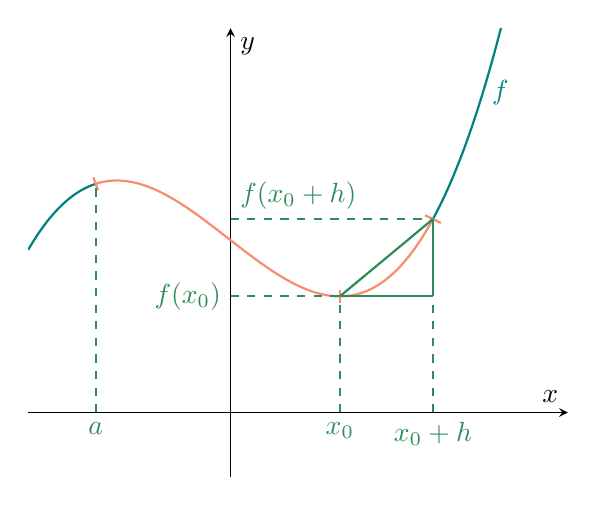
\begin{tikzpicture}
	\begin{axis}[
	axis lines = center, 
	xlabel = $x$, ylabel = $y$, 
	xmin = -3, xmax = 5, 
	ymin = -1, ymax = 6,
	ticks = none, 
	]
		\addplot[color = teal, thick, domain = -3:-2, samples = 500] {0.1*x^(3) + 0.01*x^(2) - 0.82*x + 2.69};
		\addplot[color = teal, thick, domain = 3:5, samples = 500] {0.1*x^(3) + 0.01*x^(2) - 0.82*x + 2.69};
		\addplot[color = Melon, thick, domain = -2:3, samples = 500] {0.1*x^(3) + 0.01*x^(2) - 0.82*x + 2.69};
		\draw[color = Melon, thick] (axis cs: {-0.34 * 0.1 - 2} , 0.1 + 3.57 ) --
		 (axis cs: {0.34 * 0.1 - 2}, -0.1 + 3.57  );
		\node[color = teal] at (axis cs: 4,5) {$f$};
		%Ticks and dashes
		\node[color = SeaGreen, anchor = north] at (axis cs: -2,0) {$a$};
		\node[color = SeaGreen, anchor = north] at (axis cs: 1.62,0) {$x_0$};
		\node[color = SeaGreen, anchor = north] at (axis cs: 3,0) {$x_0 + h$};
		\node[color = SeaGreen, anchor = east] at (axis cs: 0,1.813) {$f(x_0)$};
		\node[color = SeaGreen, anchor = south west] at (axis cs: 0,3.02) {$f(x_0 + h)$};
		\draw[color = SeaGreen, dashed, thick] (axis cs: -2,0) -- (axis cs: -2,3.57);
		\draw[color = SeaGreen, dashed, thick] (axis cs: 1.62,0) -- (axis cs: 1.62,1.813);
		\draw[color = SeaGreen, dashed, thick] (axis cs: 3,0) -- (axis cs: 3,3.02);
		\draw[color = SeaGreen, dashed, thick] (axis cs: 0,1.813) -- (axis cs: 1.62,1.813);
		\draw[color = SeaGreen, dashed, thick] (axis cs: 0,3.02) -- (axis cs: 3,3.02);
		%
		\draw[color = Melon, thick] (axis cs: 1.62 , 1.813 + 0.1) --
		 (axis cs: 1.62, 1.813 - 0.1);
		 \draw[color = Melon, thick] (axis cs: {-1.94 * 0.06 + 3} , 0.06 + 3.02 ) --
		 (axis cs: {1.94 * 0.06 + 3}, -0.06 + 3.02);
		%Triangle
		\draw[color = SeaGreen, thick] (axis cs: 1.62,1.813) -- (axis cs: 3,3.02);
		\draw[color = SeaGreen, thick] (axis cs: 1.62,1.813) -- (axis cs: 3,1.813);
		\draw[color = SeaGreen, thick] (axis cs: 3,1.813) -- (axis cs: 3,3.02);
	\end{axis}
	\end{tikzpicture}
	\caption{Approksimation af kurvelængde med ret linje.}
	\label{fig:kurvebevis}
	\end{figure}
Vi kalder kurvelængdefunktionen, der giver kurvelængden for $f$ på intervallet $a$ til $x$ for $L_a(x)$. 
\begin{enumerate}[label=\roman*)]
	\item Brug Pythagoras' sætning til at bestemme længden af hypotenusen for trekanten på Figur \ref{fig:kurvebevis}.
	\item Argumenter for, at vi kan lave følgende approksimation
	\begin{align*}
		L_a(x_0 + h) \approx L_a(x_0) + |\textnormal{hyp}|.
	\end{align*}
	\item Træk $L_a(x_0)$ Fra i approksimationen. 
	\item Divider udtrykket med $h$. 
	\item Brug potens- og brøkregneregler til at omskrive højresiden til
	\begin{align*}
		\sqrt{1 + \left(\frac{f(x_0 + h)-f(x_0)}{h}\right)^2}.
	\end{align*}
	\item Lad $h \to 0$. 
	\item Argumentér for, at $L_a(x)$ er en stamfunktion til $\sqrt{1 + (f'(x))^2}$.
	\item Brug denne stamfunktion på 
	$$\int_a^b \sqrt{1 + (f'(x))^2} dx$$
	 og sæt firkanten. 
\end{enumerate}